\documentclass[11pt]{article}

    \usepackage[breakable]{tcolorbox}
    \usepackage{parskip} % Stop auto-indenting (to mimic markdown behaviour)
    
    \usepackage{iftex}
    \ifPDFTeX
    	\usepackage[T1]{fontenc}
    	\usepackage{mathpazo}
    \else
    	\usepackage{fontspec}
    \fi

    % Basic figure setup, for now with no caption control since it's done
    % automatically by Pandoc (which extracts ![](path) syntax from Markdown).
    \usepackage{graphicx}
    % Maintain compatibility with old templates. Remove in nbconvert 6.0
    \let\Oldincludegraphics\includegraphics
    % Ensure that by default, figures have no caption (until we provide a
    % proper Figure object with a Caption API and a way to capture that
    % in the conversion process - todo).
    \usepackage{caption}
    \DeclareCaptionFormat{nocaption}{}
    \captionsetup{format=nocaption,aboveskip=0pt,belowskip=0pt}

    \usepackage[Export]{adjustbox} % Used to constrain images to a maximum size
    \adjustboxset{max size={0.9\linewidth}{0.9\paperheight}}
    \usepackage{float}
    \floatplacement{figure}{H} % forces figures to be placed at the correct location
    \usepackage{xcolor} % Allow colors to be defined
    \usepackage{enumerate} % Needed for markdown enumerations to work
    \usepackage{geometry} % Used to adjust the document margins
    \usepackage{amsmath} % Equations
    \usepackage{amssymb} % Equations
    \usepackage{textcomp} % defines textquotesingle
    % Hack from http://tex.stackexchange.com/a/47451/13684:
    \AtBeginDocument{%
        \def\PYZsq{\textquotesingle}% Upright quotes in Pygmentized code
    }
    \usepackage{upquote} % Upright quotes for verbatim code
    \usepackage{eurosym} % defines \euro
    \usepackage[mathletters]{ucs} % Extended unicode (utf-8) support
    \usepackage{fancyvrb} % verbatim replacement that allows latex
    \usepackage{grffile} % extends the file name processing of package graphics 
                         % to support a larger range
    \makeatletter % fix for grffile with XeLaTeX
    \def\Gread@@xetex#1{%
      \IfFileExists{"\Gin@base".bb}%
      {\Gread@eps{\Gin@base.bb}}%
      {\Gread@@xetex@aux#1}%
    }
    \makeatother

    % The hyperref package gives us a pdf with properly built
    % internal navigation ('pdf bookmarks' for the table of contents,
    % internal cross-reference links, web links for URLs, etc.)
    \usepackage{hyperref}
    % The default LaTeX title has an obnoxious amount of whitespace. By default,
    % titling removes some of it. It also provides customization options.
    \usepackage{titling}
    \usepackage{longtable} % longtable support required by pandoc >1.10
    \usepackage{booktabs}  % table support for pandoc > 1.12.2
    \usepackage[inline]{enumitem} % IRkernel/repr support (it uses the enumerate* environment)
    \usepackage[normalem]{ulem} % ulem is needed to support strikethroughs (\sout)
                                % normalem makes italics be italics, not underlines
    \usepackage{mathrsfs}
    

    
    % Colors for the hyperref package
    \definecolor{urlcolor}{rgb}{0,.145,.698}
    \definecolor{linkcolor}{rgb}{.71,0.21,0.01}
    \definecolor{citecolor}{rgb}{.12,.54,.11}

    % ANSI colors
    \definecolor{ansi-black}{HTML}{3E424D}
    \definecolor{ansi-black-intense}{HTML}{282C36}
    \definecolor{ansi-red}{HTML}{E75C58}
    \definecolor{ansi-red-intense}{HTML}{B22B31}
    \definecolor{ansi-green}{HTML}{00A250}
    \definecolor{ansi-green-intense}{HTML}{007427}
    \definecolor{ansi-yellow}{HTML}{DDB62B}
    \definecolor{ansi-yellow-intense}{HTML}{B27D12}
    \definecolor{ansi-blue}{HTML}{208FFB}
    \definecolor{ansi-blue-intense}{HTML}{0065CA}
    \definecolor{ansi-magenta}{HTML}{D160C4}
    \definecolor{ansi-magenta-intense}{HTML}{A03196}
    \definecolor{ansi-cyan}{HTML}{60C6C8}
    \definecolor{ansi-cyan-intense}{HTML}{258F8F}
    \definecolor{ansi-white}{HTML}{C5C1B4}
    \definecolor{ansi-white-intense}{HTML}{A1A6B2}
    \definecolor{ansi-default-inverse-fg}{HTML}{FFFFFF}
    \definecolor{ansi-default-inverse-bg}{HTML}{000000}

    % commands and environments needed by pandoc snippets
    % extracted from the output of `pandoc -s`
    \providecommand{\tightlist}{%
      \setlength{\itemsep}{0pt}\setlength{\parskip}{0pt}}
    \DefineVerbatimEnvironment{Highlighting}{Verbatim}{commandchars=\\\{\}}
    % Add ',fontsize=\small' for more characters per line
    \newenvironment{Shaded}{}{}
    \newcommand{\KeywordTok}[1]{\textcolor[rgb]{0.00,0.44,0.13}{\textbf{{#1}}}}
    \newcommand{\DataTypeTok}[1]{\textcolor[rgb]{0.56,0.13,0.00}{{#1}}}
    \newcommand{\DecValTok}[1]{\textcolor[rgb]{0.25,0.63,0.44}{{#1}}}
    \newcommand{\BaseNTok}[1]{\textcolor[rgb]{0.25,0.63,0.44}{{#1}}}
    \newcommand{\FloatTok}[1]{\textcolor[rgb]{0.25,0.63,0.44}{{#1}}}
    \newcommand{\CharTok}[1]{\textcolor[rgb]{0.25,0.44,0.63}{{#1}}}
    \newcommand{\StringTok}[1]{\textcolor[rgb]{0.25,0.44,0.63}{{#1}}}
    \newcommand{\CommentTok}[1]{\textcolor[rgb]{0.38,0.63,0.69}{\textit{{#1}}}}
    \newcommand{\OtherTok}[1]{\textcolor[rgb]{0.00,0.44,0.13}{{#1}}}
    \newcommand{\AlertTok}[1]{\textcolor[rgb]{1.00,0.00,0.00}{\textbf{{#1}}}}
    \newcommand{\FunctionTok}[1]{\textcolor[rgb]{0.02,0.16,0.49}{{#1}}}
    \newcommand{\RegionMarkerTok}[1]{{#1}}
    \newcommand{\ErrorTok}[1]{\textcolor[rgb]{1.00,0.00,0.00}{\textbf{{#1}}}}
    \newcommand{\NormalTok}[1]{{#1}}
    
    % Additional commands for more recent versions of Pandoc
    \newcommand{\ConstantTok}[1]{\textcolor[rgb]{0.53,0.00,0.00}{{#1}}}
    \newcommand{\SpecialCharTok}[1]{\textcolor[rgb]{0.25,0.44,0.63}{{#1}}}
    \newcommand{\VerbatimStringTok}[1]{\textcolor[rgb]{0.25,0.44,0.63}{{#1}}}
    \newcommand{\SpecialStringTok}[1]{\textcolor[rgb]{0.73,0.40,0.53}{{#1}}}
    \newcommand{\ImportTok}[1]{{#1}}
    \newcommand{\DocumentationTok}[1]{\textcolor[rgb]{0.73,0.13,0.13}{\textit{{#1}}}}
    \newcommand{\AnnotationTok}[1]{\textcolor[rgb]{0.38,0.63,0.69}{\textbf{\textit{{#1}}}}}
    \newcommand{\CommentVarTok}[1]{\textcolor[rgb]{0.38,0.63,0.69}{\textbf{\textit{{#1}}}}}
    \newcommand{\VariableTok}[1]{\textcolor[rgb]{0.10,0.09,0.49}{{#1}}}
    \newcommand{\ControlFlowTok}[1]{\textcolor[rgb]{0.00,0.44,0.13}{\textbf{{#1}}}}
    \newcommand{\OperatorTok}[1]{\textcolor[rgb]{0.40,0.40,0.40}{{#1}}}
    \newcommand{\BuiltInTok}[1]{{#1}}
    \newcommand{\ExtensionTok}[1]{{#1}}
    \newcommand{\PreprocessorTok}[1]{\textcolor[rgb]{0.74,0.48,0.00}{{#1}}}
    \newcommand{\AttributeTok}[1]{\textcolor[rgb]{0.49,0.56,0.16}{{#1}}}
    \newcommand{\InformationTok}[1]{\textcolor[rgb]{0.38,0.63,0.69}{\textbf{\textit{{#1}}}}}
    \newcommand{\WarningTok}[1]{\textcolor[rgb]{0.38,0.63,0.69}{\textbf{\textit{{#1}}}}}
    
    
    % Define a nice break command that doesn't care if a line doesn't already
    % exist.
    \def\br{\hspace*{\fill} \\* }
    % Math Jax compatibility definitions
    \def\gt{>}
    \def\lt{<}
    \let\Oldtex\TeX
    \let\Oldlatex\LaTeX
    \renewcommand{\TeX}{\textrm{\Oldtex}}
    \renewcommand{\LaTeX}{\textrm{\Oldlatex}}
    % Document parameters
    % Document title
    \title{SignalKInputStreamer}
    
    
    
    
    
% Pygments definitions
\makeatletter
\def\PY@reset{\let\PY@it=\relax \let\PY@bf=\relax%
    \let\PY@ul=\relax \let\PY@tc=\relax%
    \let\PY@bc=\relax \let\PY@ff=\relax}
\def\PY@tok#1{\csname PY@tok@#1\endcsname}
\def\PY@toks#1+{\ifx\relax#1\empty\else%
    \PY@tok{#1}\expandafter\PY@toks\fi}
\def\PY@do#1{\PY@bc{\PY@tc{\PY@ul{%
    \PY@it{\PY@bf{\PY@ff{#1}}}}}}}
\def\PY#1#2{\PY@reset\PY@toks#1+\relax+\PY@do{#2}}

\expandafter\def\csname PY@tok@w\endcsname{\def\PY@tc##1{\textcolor[rgb]{0.73,0.73,0.73}{##1}}}
\expandafter\def\csname PY@tok@c\endcsname{\let\PY@it=\textit\def\PY@tc##1{\textcolor[rgb]{0.25,0.50,0.50}{##1}}}
\expandafter\def\csname PY@tok@cp\endcsname{\def\PY@tc##1{\textcolor[rgb]{0.74,0.48,0.00}{##1}}}
\expandafter\def\csname PY@tok@k\endcsname{\let\PY@bf=\textbf\def\PY@tc##1{\textcolor[rgb]{0.00,0.50,0.00}{##1}}}
\expandafter\def\csname PY@tok@kp\endcsname{\def\PY@tc##1{\textcolor[rgb]{0.00,0.50,0.00}{##1}}}
\expandafter\def\csname PY@tok@kt\endcsname{\def\PY@tc##1{\textcolor[rgb]{0.69,0.00,0.25}{##1}}}
\expandafter\def\csname PY@tok@o\endcsname{\def\PY@tc##1{\textcolor[rgb]{0.40,0.40,0.40}{##1}}}
\expandafter\def\csname PY@tok@ow\endcsname{\let\PY@bf=\textbf\def\PY@tc##1{\textcolor[rgb]{0.67,0.13,1.00}{##1}}}
\expandafter\def\csname PY@tok@nb\endcsname{\def\PY@tc##1{\textcolor[rgb]{0.00,0.50,0.00}{##1}}}
\expandafter\def\csname PY@tok@nf\endcsname{\def\PY@tc##1{\textcolor[rgb]{0.00,0.00,1.00}{##1}}}
\expandafter\def\csname PY@tok@nc\endcsname{\let\PY@bf=\textbf\def\PY@tc##1{\textcolor[rgb]{0.00,0.00,1.00}{##1}}}
\expandafter\def\csname PY@tok@nn\endcsname{\let\PY@bf=\textbf\def\PY@tc##1{\textcolor[rgb]{0.00,0.00,1.00}{##1}}}
\expandafter\def\csname PY@tok@ne\endcsname{\let\PY@bf=\textbf\def\PY@tc##1{\textcolor[rgb]{0.82,0.25,0.23}{##1}}}
\expandafter\def\csname PY@tok@nv\endcsname{\def\PY@tc##1{\textcolor[rgb]{0.10,0.09,0.49}{##1}}}
\expandafter\def\csname PY@tok@no\endcsname{\def\PY@tc##1{\textcolor[rgb]{0.53,0.00,0.00}{##1}}}
\expandafter\def\csname PY@tok@nl\endcsname{\def\PY@tc##1{\textcolor[rgb]{0.63,0.63,0.00}{##1}}}
\expandafter\def\csname PY@tok@ni\endcsname{\let\PY@bf=\textbf\def\PY@tc##1{\textcolor[rgb]{0.60,0.60,0.60}{##1}}}
\expandafter\def\csname PY@tok@na\endcsname{\def\PY@tc##1{\textcolor[rgb]{0.49,0.56,0.16}{##1}}}
\expandafter\def\csname PY@tok@nt\endcsname{\let\PY@bf=\textbf\def\PY@tc##1{\textcolor[rgb]{0.00,0.50,0.00}{##1}}}
\expandafter\def\csname PY@tok@nd\endcsname{\def\PY@tc##1{\textcolor[rgb]{0.67,0.13,1.00}{##1}}}
\expandafter\def\csname PY@tok@s\endcsname{\def\PY@tc##1{\textcolor[rgb]{0.73,0.13,0.13}{##1}}}
\expandafter\def\csname PY@tok@sd\endcsname{\let\PY@it=\textit\def\PY@tc##1{\textcolor[rgb]{0.73,0.13,0.13}{##1}}}
\expandafter\def\csname PY@tok@si\endcsname{\let\PY@bf=\textbf\def\PY@tc##1{\textcolor[rgb]{0.73,0.40,0.53}{##1}}}
\expandafter\def\csname PY@tok@se\endcsname{\let\PY@bf=\textbf\def\PY@tc##1{\textcolor[rgb]{0.73,0.40,0.13}{##1}}}
\expandafter\def\csname PY@tok@sr\endcsname{\def\PY@tc##1{\textcolor[rgb]{0.73,0.40,0.53}{##1}}}
\expandafter\def\csname PY@tok@ss\endcsname{\def\PY@tc##1{\textcolor[rgb]{0.10,0.09,0.49}{##1}}}
\expandafter\def\csname PY@tok@sx\endcsname{\def\PY@tc##1{\textcolor[rgb]{0.00,0.50,0.00}{##1}}}
\expandafter\def\csname PY@tok@m\endcsname{\def\PY@tc##1{\textcolor[rgb]{0.40,0.40,0.40}{##1}}}
\expandafter\def\csname PY@tok@gh\endcsname{\let\PY@bf=\textbf\def\PY@tc##1{\textcolor[rgb]{0.00,0.00,0.50}{##1}}}
\expandafter\def\csname PY@tok@gu\endcsname{\let\PY@bf=\textbf\def\PY@tc##1{\textcolor[rgb]{0.50,0.00,0.50}{##1}}}
\expandafter\def\csname PY@tok@gd\endcsname{\def\PY@tc##1{\textcolor[rgb]{0.63,0.00,0.00}{##1}}}
\expandafter\def\csname PY@tok@gi\endcsname{\def\PY@tc##1{\textcolor[rgb]{0.00,0.63,0.00}{##1}}}
\expandafter\def\csname PY@tok@gr\endcsname{\def\PY@tc##1{\textcolor[rgb]{1.00,0.00,0.00}{##1}}}
\expandafter\def\csname PY@tok@ge\endcsname{\let\PY@it=\textit}
\expandafter\def\csname PY@tok@gs\endcsname{\let\PY@bf=\textbf}
\expandafter\def\csname PY@tok@gp\endcsname{\let\PY@bf=\textbf\def\PY@tc##1{\textcolor[rgb]{0.00,0.00,0.50}{##1}}}
\expandafter\def\csname PY@tok@go\endcsname{\def\PY@tc##1{\textcolor[rgb]{0.53,0.53,0.53}{##1}}}
\expandafter\def\csname PY@tok@gt\endcsname{\def\PY@tc##1{\textcolor[rgb]{0.00,0.27,0.87}{##1}}}
\expandafter\def\csname PY@tok@err\endcsname{\def\PY@bc##1{\setlength{\fboxsep}{0pt}\fcolorbox[rgb]{1.00,0.00,0.00}{1,1,1}{\strut ##1}}}
\expandafter\def\csname PY@tok@kc\endcsname{\let\PY@bf=\textbf\def\PY@tc##1{\textcolor[rgb]{0.00,0.50,0.00}{##1}}}
\expandafter\def\csname PY@tok@kd\endcsname{\let\PY@bf=\textbf\def\PY@tc##1{\textcolor[rgb]{0.00,0.50,0.00}{##1}}}
\expandafter\def\csname PY@tok@kn\endcsname{\let\PY@bf=\textbf\def\PY@tc##1{\textcolor[rgb]{0.00,0.50,0.00}{##1}}}
\expandafter\def\csname PY@tok@kr\endcsname{\let\PY@bf=\textbf\def\PY@tc##1{\textcolor[rgb]{0.00,0.50,0.00}{##1}}}
\expandafter\def\csname PY@tok@bp\endcsname{\def\PY@tc##1{\textcolor[rgb]{0.00,0.50,0.00}{##1}}}
\expandafter\def\csname PY@tok@fm\endcsname{\def\PY@tc##1{\textcolor[rgb]{0.00,0.00,1.00}{##1}}}
\expandafter\def\csname PY@tok@vc\endcsname{\def\PY@tc##1{\textcolor[rgb]{0.10,0.09,0.49}{##1}}}
\expandafter\def\csname PY@tok@vg\endcsname{\def\PY@tc##1{\textcolor[rgb]{0.10,0.09,0.49}{##1}}}
\expandafter\def\csname PY@tok@vi\endcsname{\def\PY@tc##1{\textcolor[rgb]{0.10,0.09,0.49}{##1}}}
\expandafter\def\csname PY@tok@vm\endcsname{\def\PY@tc##1{\textcolor[rgb]{0.10,0.09,0.49}{##1}}}
\expandafter\def\csname PY@tok@sa\endcsname{\def\PY@tc##1{\textcolor[rgb]{0.73,0.13,0.13}{##1}}}
\expandafter\def\csname PY@tok@sb\endcsname{\def\PY@tc##1{\textcolor[rgb]{0.73,0.13,0.13}{##1}}}
\expandafter\def\csname PY@tok@sc\endcsname{\def\PY@tc##1{\textcolor[rgb]{0.73,0.13,0.13}{##1}}}
\expandafter\def\csname PY@tok@dl\endcsname{\def\PY@tc##1{\textcolor[rgb]{0.73,0.13,0.13}{##1}}}
\expandafter\def\csname PY@tok@s2\endcsname{\def\PY@tc##1{\textcolor[rgb]{0.73,0.13,0.13}{##1}}}
\expandafter\def\csname PY@tok@sh\endcsname{\def\PY@tc##1{\textcolor[rgb]{0.73,0.13,0.13}{##1}}}
\expandafter\def\csname PY@tok@s1\endcsname{\def\PY@tc##1{\textcolor[rgb]{0.73,0.13,0.13}{##1}}}
\expandafter\def\csname PY@tok@mb\endcsname{\def\PY@tc##1{\textcolor[rgb]{0.40,0.40,0.40}{##1}}}
\expandafter\def\csname PY@tok@mf\endcsname{\def\PY@tc##1{\textcolor[rgb]{0.40,0.40,0.40}{##1}}}
\expandafter\def\csname PY@tok@mh\endcsname{\def\PY@tc##1{\textcolor[rgb]{0.40,0.40,0.40}{##1}}}
\expandafter\def\csname PY@tok@mi\endcsname{\def\PY@tc##1{\textcolor[rgb]{0.40,0.40,0.40}{##1}}}
\expandafter\def\csname PY@tok@il\endcsname{\def\PY@tc##1{\textcolor[rgb]{0.40,0.40,0.40}{##1}}}
\expandafter\def\csname PY@tok@mo\endcsname{\def\PY@tc##1{\textcolor[rgb]{0.40,0.40,0.40}{##1}}}
\expandafter\def\csname PY@tok@ch\endcsname{\let\PY@it=\textit\def\PY@tc##1{\textcolor[rgb]{0.25,0.50,0.50}{##1}}}
\expandafter\def\csname PY@tok@cm\endcsname{\let\PY@it=\textit\def\PY@tc##1{\textcolor[rgb]{0.25,0.50,0.50}{##1}}}
\expandafter\def\csname PY@tok@cpf\endcsname{\let\PY@it=\textit\def\PY@tc##1{\textcolor[rgb]{0.25,0.50,0.50}{##1}}}
\expandafter\def\csname PY@tok@c1\endcsname{\let\PY@it=\textit\def\PY@tc##1{\textcolor[rgb]{0.25,0.50,0.50}{##1}}}
\expandafter\def\csname PY@tok@cs\endcsname{\let\PY@it=\textit\def\PY@tc##1{\textcolor[rgb]{0.25,0.50,0.50}{##1}}}

\def\PYZbs{\char`\\}
\def\PYZus{\char`\_}
\def\PYZob{\char`\{}
\def\PYZcb{\char`\}}
\def\PYZca{\char`\^}
\def\PYZam{\char`\&}
\def\PYZlt{\char`\<}
\def\PYZgt{\char`\>}
\def\PYZsh{\char`\#}
\def\PYZpc{\char`\%}
\def\PYZdl{\char`\$}
\def\PYZhy{\char`\-}
\def\PYZsq{\char`\'}
\def\PYZdq{\char`\"}
\def\PYZti{\char`\~}
% for compatibility with earlier versions
\def\PYZat{@}
\def\PYZlb{[}
\def\PYZrb{]}
\makeatother


    % For linebreaks inside Verbatim environment from package fancyvrb. 
    \makeatletter
        \newbox\Wrappedcontinuationbox 
        \newbox\Wrappedvisiblespacebox 
        \newcommand*\Wrappedvisiblespace {\textcolor{red}{\textvisiblespace}} 
        \newcommand*\Wrappedcontinuationsymbol {\textcolor{red}{\llap{\tiny$\m@th\hookrightarrow$}}} 
        \newcommand*\Wrappedcontinuationindent {3ex } 
        \newcommand*\Wrappedafterbreak {\kern\Wrappedcontinuationindent\copy\Wrappedcontinuationbox} 
        % Take advantage of the already applied Pygments mark-up to insert 
        % potential linebreaks for TeX processing. 
        %        {, <, #, %, $, ' and ": go to next line. 
        %        _, }, ^, &, >, - and ~: stay at end of broken line. 
        % Use of \textquotesingle for straight quote. 
        \newcommand*\Wrappedbreaksatspecials {% 
            \def\PYGZus{\discretionary{\char`\_}{\Wrappedafterbreak}{\char`\_}}% 
            \def\PYGZob{\discretionary{}{\Wrappedafterbreak\char`\{}{\char`\{}}% 
            \def\PYGZcb{\discretionary{\char`\}}{\Wrappedafterbreak}{\char`\}}}% 
            \def\PYGZca{\discretionary{\char`\^}{\Wrappedafterbreak}{\char`\^}}% 
            \def\PYGZam{\discretionary{\char`\&}{\Wrappedafterbreak}{\char`\&}}% 
            \def\PYGZlt{\discretionary{}{\Wrappedafterbreak\char`\<}{\char`\<}}% 
            \def\PYGZgt{\discretionary{\char`\>}{\Wrappedafterbreak}{\char`\>}}% 
            \def\PYGZsh{\discretionary{}{\Wrappedafterbreak\char`\#}{\char`\#}}% 
            \def\PYGZpc{\discretionary{}{\Wrappedafterbreak\char`\%}{\char`\%}}% 
            \def\PYGZdl{\discretionary{}{\Wrappedafterbreak\char`\$}{\char`\$}}% 
            \def\PYGZhy{\discretionary{\char`\-}{\Wrappedafterbreak}{\char`\-}}% 
            \def\PYGZsq{\discretionary{}{\Wrappedafterbreak\textquotesingle}{\textquotesingle}}% 
            \def\PYGZdq{\discretionary{}{\Wrappedafterbreak\char`\"}{\char`\"}}% 
            \def\PYGZti{\discretionary{\char`\~}{\Wrappedafterbreak}{\char`\~}}% 
        } 
        % Some characters . , ; ? ! / are not pygmentized. 
        % This macro makes them "active" and they will insert potential linebreaks 
        \newcommand*\Wrappedbreaksatpunct {% 
            \lccode`\~`\.\lowercase{\def~}{\discretionary{\hbox{\char`\.}}{\Wrappedafterbreak}{\hbox{\char`\.}}}% 
            \lccode`\~`\,\lowercase{\def~}{\discretionary{\hbox{\char`\,}}{\Wrappedafterbreak}{\hbox{\char`\,}}}% 
            \lccode`\~`\;\lowercase{\def~}{\discretionary{\hbox{\char`\;}}{\Wrappedafterbreak}{\hbox{\char`\;}}}% 
            \lccode`\~`\:\lowercase{\def~}{\discretionary{\hbox{\char`\:}}{\Wrappedafterbreak}{\hbox{\char`\:}}}% 
            \lccode`\~`\?\lowercase{\def~}{\discretionary{\hbox{\char`\?}}{\Wrappedafterbreak}{\hbox{\char`\?}}}% 
            \lccode`\~`\!\lowercase{\def~}{\discretionary{\hbox{\char`\!}}{\Wrappedafterbreak}{\hbox{\char`\!}}}% 
            \lccode`\~`\/\lowercase{\def~}{\discretionary{\hbox{\char`\/}}{\Wrappedafterbreak}{\hbox{\char`\/}}}% 
            \catcode`\.\active
            \catcode`\,\active 
            \catcode`\;\active
            \catcode`\:\active
            \catcode`\?\active
            \catcode`\!\active
            \catcode`\/\active 
            \lccode`\~`\~ 	
        }
    \makeatother

    \let\OriginalVerbatim=\Verbatim
    \makeatletter
    \renewcommand{\Verbatim}[1][1]{%
        %\parskip\z@skip
        \sbox\Wrappedcontinuationbox {\Wrappedcontinuationsymbol}%
        \sbox\Wrappedvisiblespacebox {\FV@SetupFont\Wrappedvisiblespace}%
        \def\FancyVerbFormatLine ##1{\hsize\linewidth
            \vtop{\raggedright\hyphenpenalty\z@\exhyphenpenalty\z@
                \doublehyphendemerits\z@\finalhyphendemerits\z@
                \strut ##1\strut}%
        }%
        % If the linebreak is at a space, the latter will be displayed as visible
        % space at end of first line, and a continuation symbol starts next line.
        % Stretch/shrink are however usually zero for typewriter font.
        \def\FV@Space {%
            \nobreak\hskip\z@ plus\fontdimen3\font minus\fontdimen4\font
            \discretionary{\copy\Wrappedvisiblespacebox}{\Wrappedafterbreak}
            {\kern\fontdimen2\font}%
        }%
        
        % Allow breaks at special characters using \PYG... macros.
        \Wrappedbreaksatspecials
        % Breaks at punctuation characters . , ; ? ! and / need catcode=\active 	
        \OriginalVerbatim[#1,codes*=\Wrappedbreaksatpunct]%
    }
    \makeatother

    % Exact colors from NB
    \definecolor{incolor}{HTML}{303F9F}
    \definecolor{outcolor}{HTML}{D84315}
    \definecolor{cellborder}{HTML}{CFCFCF}
    \definecolor{cellbackground}{HTML}{F7F7F7}
    
    % prompt
    \makeatletter
    \newcommand{\boxspacing}{\kern\kvtcb@left@rule\kern\kvtcb@boxsep}
    \makeatother
    \newcommand{\prompt}[4]{
        \ttfamily\llap{{\color{#2}[#3]:\hspace{3pt}#4}}\vspace{-\baselineskip}
    }
    

    
    % Prevent overflowing lines due to hard-to-break entities
    \sloppy 
    % Setup hyperref package
    \hypersetup{
      breaklinks=true,  % so long urls are correctly broken across lines
      colorlinks=true,
      urlcolor=urlcolor,
      linkcolor=linkcolor,
      citecolor=citecolor,
      }
    % Slightly bigger margins than the latex defaults
    
    \geometry{verbose,tmargin=1in,bmargin=1in,lmargin=1in,rmargin=1in}
    
    

\begin{document}
    
    \maketitle
    
    

    
    \hypertarget{signal-k-input-streamer---system-design-description}{%
\section{Signal K input streamer - System Design
Description}\label{signal-k-input-streamer---system-design-description}}

    You have probably already used or got interested in
\href{https://signalk.org/overview.html}{Signal K}, the free and open
source marine data exchange format. If not, let's hope that that the
Signal K input streamer in Dashboard-Tactics plug-in of OpenCPN gets you
motivated to start moving your boat's instrumentation from 1990's to
2020's!

You may want to skip the theory and move directly to the \emph{Signal K
input streamer usage} document
(\href{SignalKInputStreamerUsage.ipynb}{ipynb} \textbar{}
\href{SignalKInputStreamerUsage.html}{html} \textbar{}
\href{SignalKInputStreamerUsage.pdf}{pdf}).

    \hypertarget{introduction}{%
\subsection{Introduction}\label{introduction}}

    The Signal K input streamer of Dashboard Tactics plug-in has been
designed to meet the following three requirements:

    \begin{enumerate}
\def\labelenumi{\arabic{enumi}.}
\tightlist
\item
  Read data in NMEA-0183, NMEA-2000 and Signal K data sources
\item
  Provide data with millisecond resolution timestamps closest to the
  data source possible
\item
  Reduce the jitter and latency from the data source to the instruments
\end{enumerate}

    Increasing of performance is out of scope - neither the Signal K input
streamer nor Dashboard Tactics pretend to miraculously increase the
throughput or multiply the update frequency of your boat's
instrumentation.

    \hypertarget{example-system-configuration}{%
\subsection{Example system
configuration}\label{example-system-configuration}}

    The below diagram illustrates an example configuration which does not
require to invest on any new hardware if one already is using TCP/IP
(network) or USB to get the NMEA-0183 data into the OpenCPN
chartplotter.

    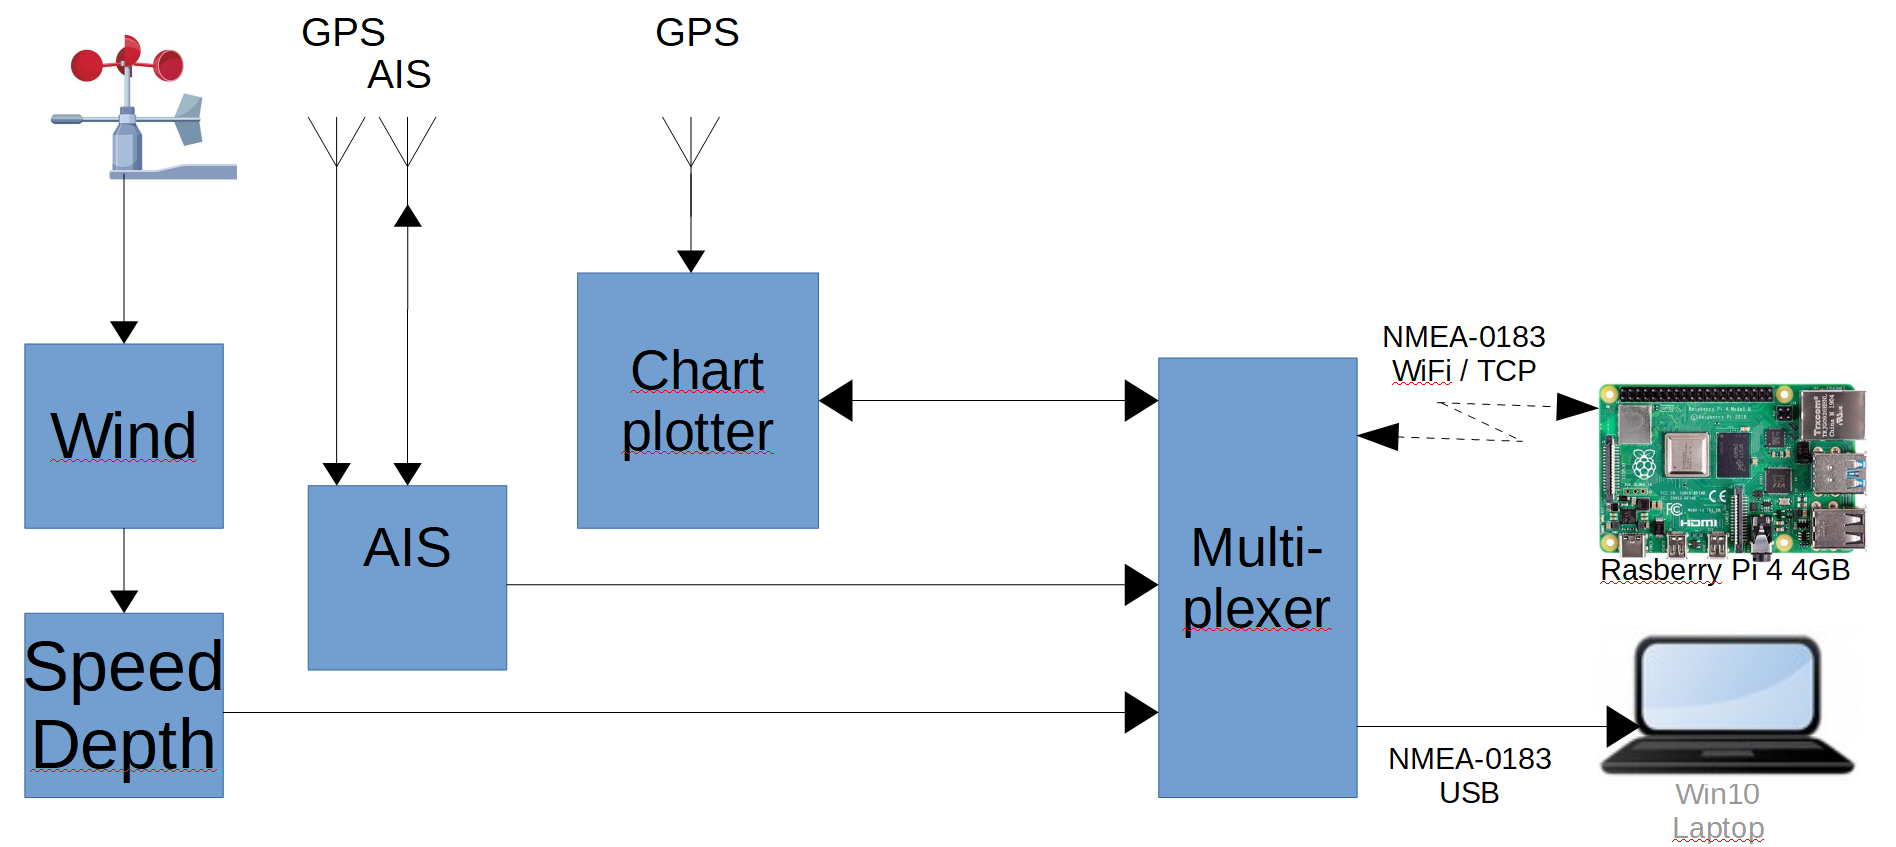
\includegraphics{signalkin-instrudiagram-1.png}
\href{img/signalkin-instrudiagram-1.png}{(zoom)}

    The Raspberry Pi 4 4G running Raspian is configured as a WiFi hotspot
while underway. A cockpit tablet (not illustrated) is used to connect to
it using a browser. Raspberry has a local screen and keyboard/trackball
on the chart table.

    The Windows 10 laptop is used as backup navigation computer and to
collect and visualize meteorological data.

    Both systems are having OpenCPN v5 with Dashboard-Tactics plug-in.

    Other such configurations exists - Signal K provides
\href{https://signalk.org/installation.html}{more examples};
\href{http://www.sailoog.com/openplotter}{OpenPlotter} project provides
entire packages containing all the necessary software components for
Debian based computers.

    \hypertarget{jitter-and-latency-in-opencpn-dashboard-data-distribution}{%
\subsection{Jitter and latency in OpenCPN / Dashboard data
distribution}\label{jitter-and-latency-in-opencpn-dashboard-data-distribution}}

    The third requirement, reduction in jitter and latency in the data
distribution is the hardest to meet. In this section we will analyze the
data signal path in OpenCPN with plug-ins and, of course in Dashboard
plug-in.

    Typically, one would need a two channel oscilloscope or accurate
timestamps from different phases of the data acquisition chain to
determine the inaccuracies in timing caused by signal chain. However,
the data in boat systems is sometime coming from systems which are so
old or based on old technologies that one can actually see the jitter
with the naked eye; values in instruments are jumping back and forth
and, very well visible in the dial instrument's needle, the frequency of
the jumping is not constant.

    It is to be reminded that it is not normal for any system which attempts
to give information about the analog world to give feedback to the user
with an indicator which is not following the real-life signal as
accurately as possible.

    Taking the example of the dial instrument's needle, it shall move so
smoothly that the eventual micro-movements are not visible to the human
eye. Furthermore, this movement shall be as accurate as possible
reflecting in real-time the actual, measured signal. Filters shall be
applied only at user's demand so that the observer is always in control.
Even if the filters are applied, it should be possible to keep both the
original data and the resulting filtered data for off-line analysis -
blind faith is not an instrumentation paradigm.

    OpenCPN / Dashboard cannot do anything for the data update frequency, it
is for the owner to update boat's instrumentation keeping in mind that
for any algorithm it is essential to have as much as possible
information about the boat's movements, its heading and wind condition
it is facing. Logically, one should seek to increase the frequency and
reduce the latency.

    OpenCPN chartplotter, Dashboard plug-in and the other plug-ins create an
extremely complicated system what comes to its dynamic behaviour. It is
not a surprise that it introduces jitter and latency in the signal chain
by its location between the user and his or her data sources, i.e.~the
boat's sensors. Of course, the boat's own electronics play an equally
important role in this, but since we cannot present an universal model
for those, let's study the signal chain from the point onwards where it
enters OpenCPN, \emph{i.e.} from USB serial line or WiFi/Ethernet TCP/IP
communication in our case.

    Below diagram illustrates the signal chain from the point of view of
Dashboard plug-in, which is the module we plan to modify.

    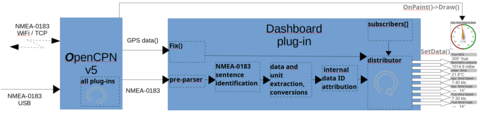
\includegraphics{signalkin-instrudiagram-2.png}
\href{img/signalkin-instrudiagram-2.png}{(zoom)}

    OpenCPN is based on \href{https://www.wxwidgets.org/}{wxWidgets}
Graphical User Interface (GUI) framework, and like many of them it is
event driven: clicking a button is an event; moving a window over
another creates events which need to be handled in both windows - an
excellent and well established principle for such a software framework.
But it is less useful for a data acquisition system unless there is a
priority scheme which allows the data event dealt with a high priority
interrupt mechanism. It should allow a continuous transport of the
arrived data all the way through the system. But if we would follow such
as principle in a graphical application, the actual GUI operation could
become sluggish and, in general the priority is given to the graphical
elements visible to user.

    OpenCPN is not a real multi-threaded in application - in the POSIX sense
of view. It is threaded using the
\href{https://docs.wxwidgets.org/trunk/classwx_thread.html}{wxWidgets
thread model} which is not POSIX compliant. It is by default serving
graphical events with what they call detached behavior. Detached threads
delete themselves once they have completed which is, of course really
useful feature in a GUI since you do not have to make call-backs or
otherwise manage the thread.

    But it is not necessarily the best adapted way to deal with socket based
communication since it can be considered to be overkilling in a
multisocket environment to launch a thread - even lightweight - for
every arriving frame in a socket, and this for every socket (\emph{i.e.}
one thread to deal with any socket ``event''). In the current user state
multi-socket server paradigm there is rather a POSIX thread per socket.
It can be specialized - a protocol handler, for example -, it is seen in
the process tables, it can have an adjustable priority, its affinity and
can be set to manage the load between the CPUs and their cores.

    Next we check that this is not the case in OpenCPN already. For the test
we use the above configuration with the exception that the Raspberry Pi
4GB running Rasbian 2019-07-10 (Buster) is serving as WiFi hotspot for
the boat's installation and the Windows 10 laptop and its OpenCPN is
obtaining both its NMEA data and AIS information from it over a wireless
TCP/IP connection with the Signal K server, running on the Raspberry
device.

    The below screenshot illustrates the threads in the Raspberry. There is
none for OpenCPN so it must be running entirely in the wxWidgets
``detached'' thread mode.

    \begin{figure}
\centering
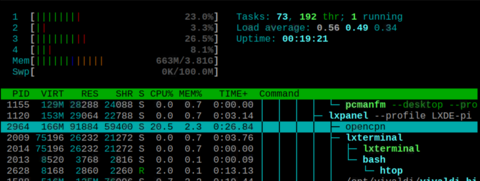
\includegraphics{2019-10-12_181939_rasbian_ov50_def_config_TCP_input_no_posix_threads.png}
\caption{2019-10-12\_181939\_rasbian\_ov50\_def\_config\_TCP\_input\_no\_posix\_threads.png}
\end{figure}

    On the Windows 10 system, the notion of POSIX threads does not exist but
the thread information can be observed with SDK tools. Like above, also
in this case we have a standard OpenCPN - Dashboard plug-in datapath for
NMEA.

    \begin{figure}
\centering
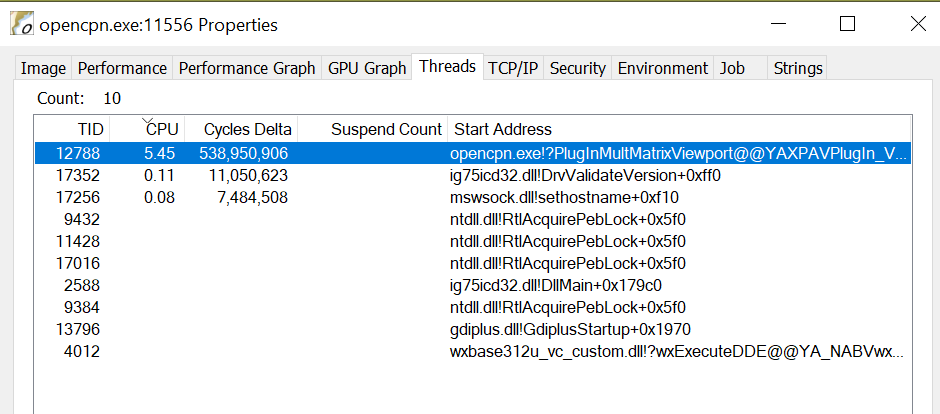
\includegraphics{2019-10-12_211524_w10_ov50_def_config_TCP_threads.png}
\caption{2019-10-12\_211524\_w10\_ov50\_def\_config\_TCP\_threads.png}
\end{figure}

    On the Windows 10 system we can see that there is plenty of capacity
available, the WiFi based NMEA / AIS information does not create any big
load to the system. The I/O load is almost insignifiant compared to the
load which occur when one mimimize/maximize the OpenCPN window, or when
it chimes the ship's bells!

    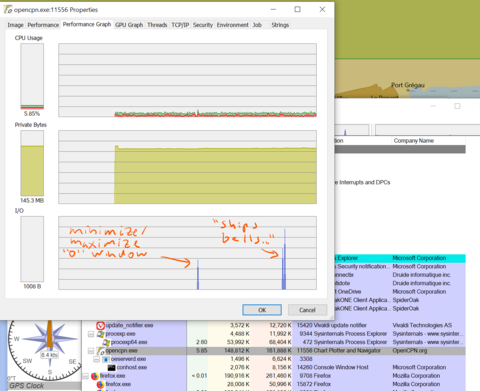
\includegraphics{2019-10-12_211525_w10_ov50_def_config_TCP_perfgraph.png}
\href{img/2019-10-12_211525_w10_ov50_def_config_TCP_perfgraph.png}{(zoom)}

    \hypertarget{threaded-model-of-the-influx-db-output-stream-service}{%
\subsubsection{Threaded model of the Influx DB output stream
service}\label{threaded-model-of-the-influx-db-output-stream-service}}

    We use the Influx DB output stream to store the results in a file with a
timestamp, generated locally. Otherwise we would have no way to define
the jitter. For the latency we cannot make the measurement since the
OpenCPN does not timestamp the data at its arrival. Therefore we will
observe the overall throughput only.

    The collected data and the results are reported later in this document.
Here we take the opportunity to study the impact of the
Dashboard-Tactics' thread model for Influx DB output in view of its
usage in the data input socket. Albeit we do not use its direct
HTTP-socket streaming capability but only the file writing, the
possibility to stream out to a HTTP-socket of the Influx DB server makes
the implementation as an attractive candidate to the input socket as
well.

    The Dashboard-Tactics' Influx DB output stream service thread, which is
implemented with wxWidgets thread model \emph{joinable} is clearly
visible in the Raspberry device, so wxWidgets has implemented it quite
probably with Linux POSIX threads:

    \begin{figure}
\centering
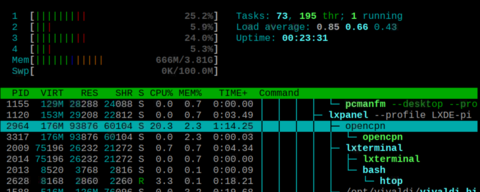
\includegraphics{2019-10-12_182337_rasbian_ov50_Influxdbout_TCP_input_1_posix_thread.png}
\caption{2019-10-12\_182337\_rasbian\_ov50\_Influxdbout\_TCP\_input\_1\_posix\_thread.png}
\end{figure}

    It is less visible in the Windows 10 thread model but one can count one
more CPU time consuming thread, clearly a wxWidgets DLL:

    \begin{figure}
\centering
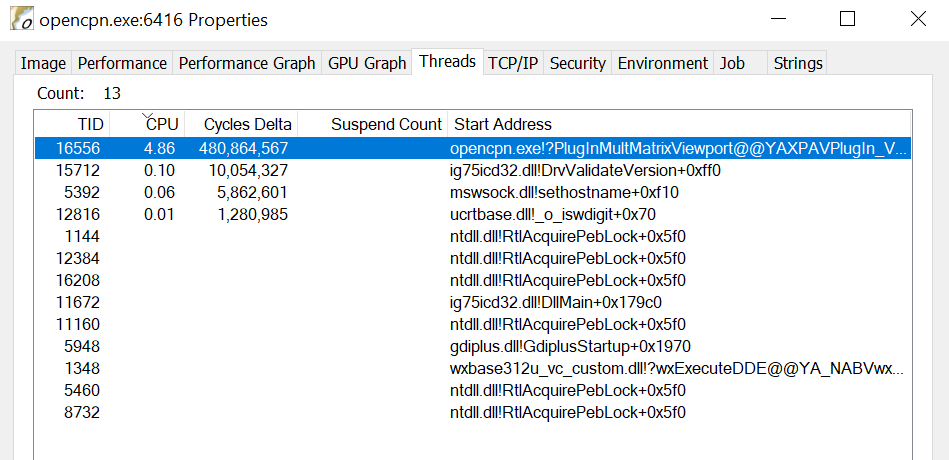
\includegraphics{2019-10-12_211425_w10_ov50_influxdbout_TCP_threads.png}
\caption{2019-10-12\_211425\_w10\_ov50\_influxdbout\_TCP\_threads.png}
\end{figure}

    The I/O system load now shows also clearly the flush-mechanism which is
built-in into the file writing part of the threaded service. The load of
the I/O operations is in the disk writes not in the network sockets.

    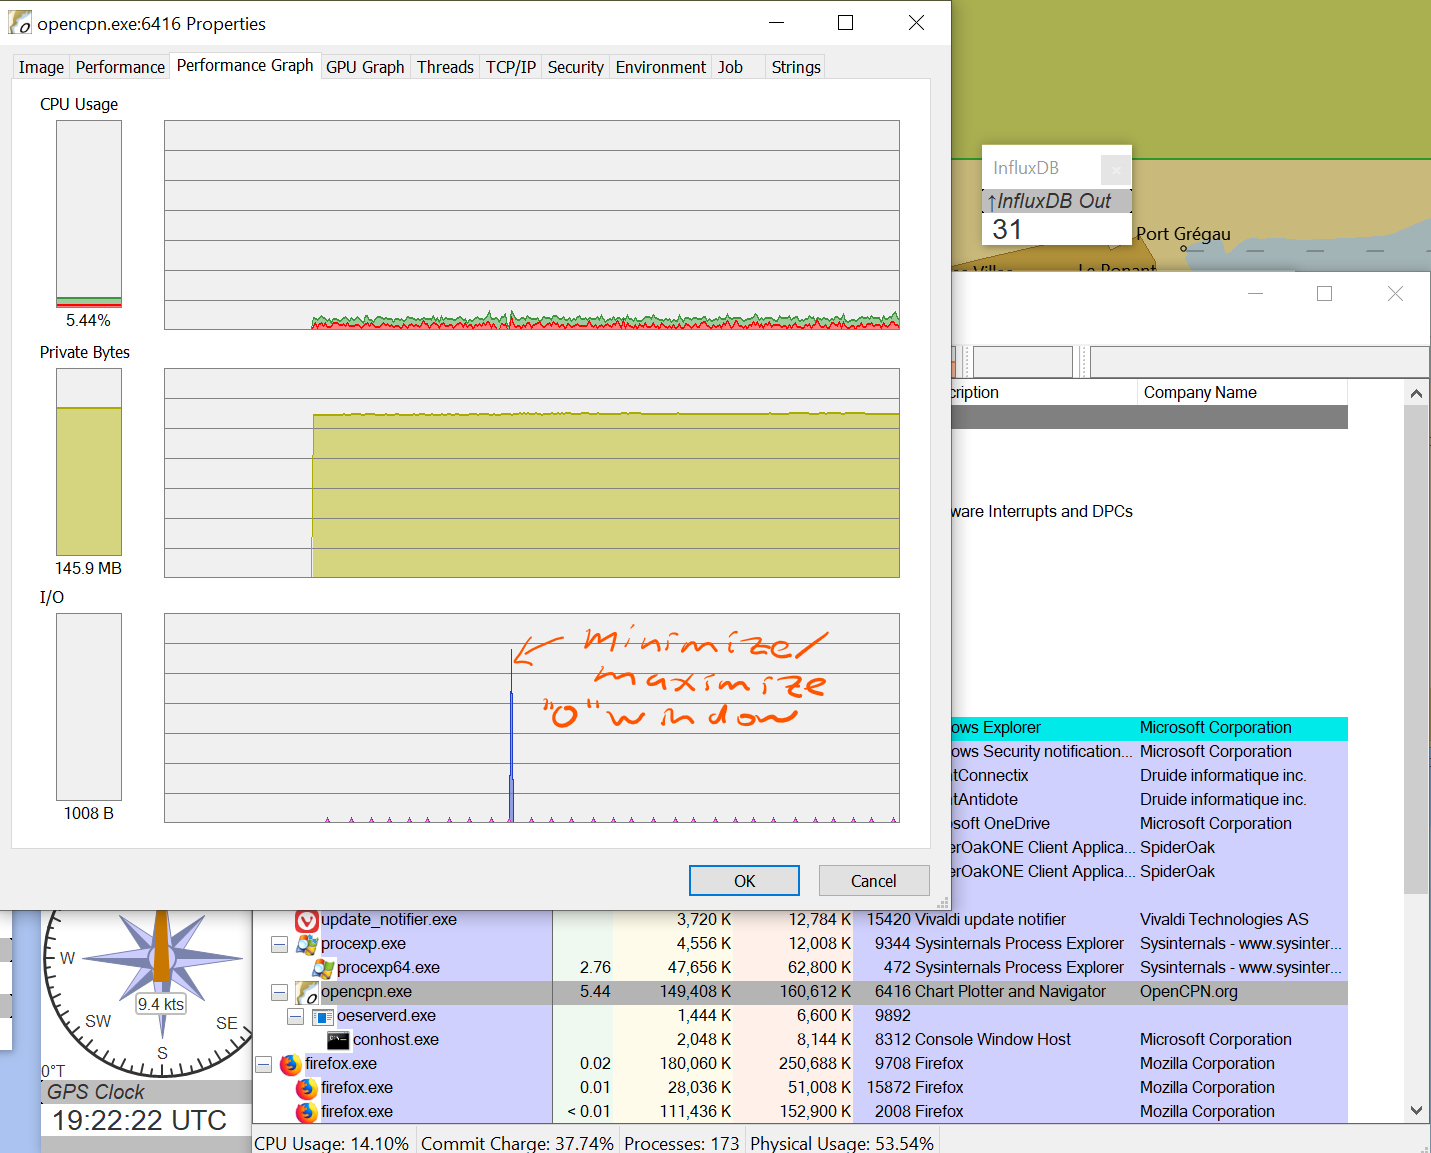
\includegraphics{2019-10-12_211425_w10_ov50_influxdbout_TCP_perfgraph.png}
\href{img/2019-10-12_211425_w10_ov50_influxdbout_TCP_perfgraph.png}{(zoom)}

    \hypertarget{system-design-of-the-signal-k-input-streamer}{%
\subsection{System design of the Signal K input
streamer}\label{system-design-of-the-signal-k-input-streamer}}

    The below diagram illustrates the system architecture with the Signal K
input streamer extension.

    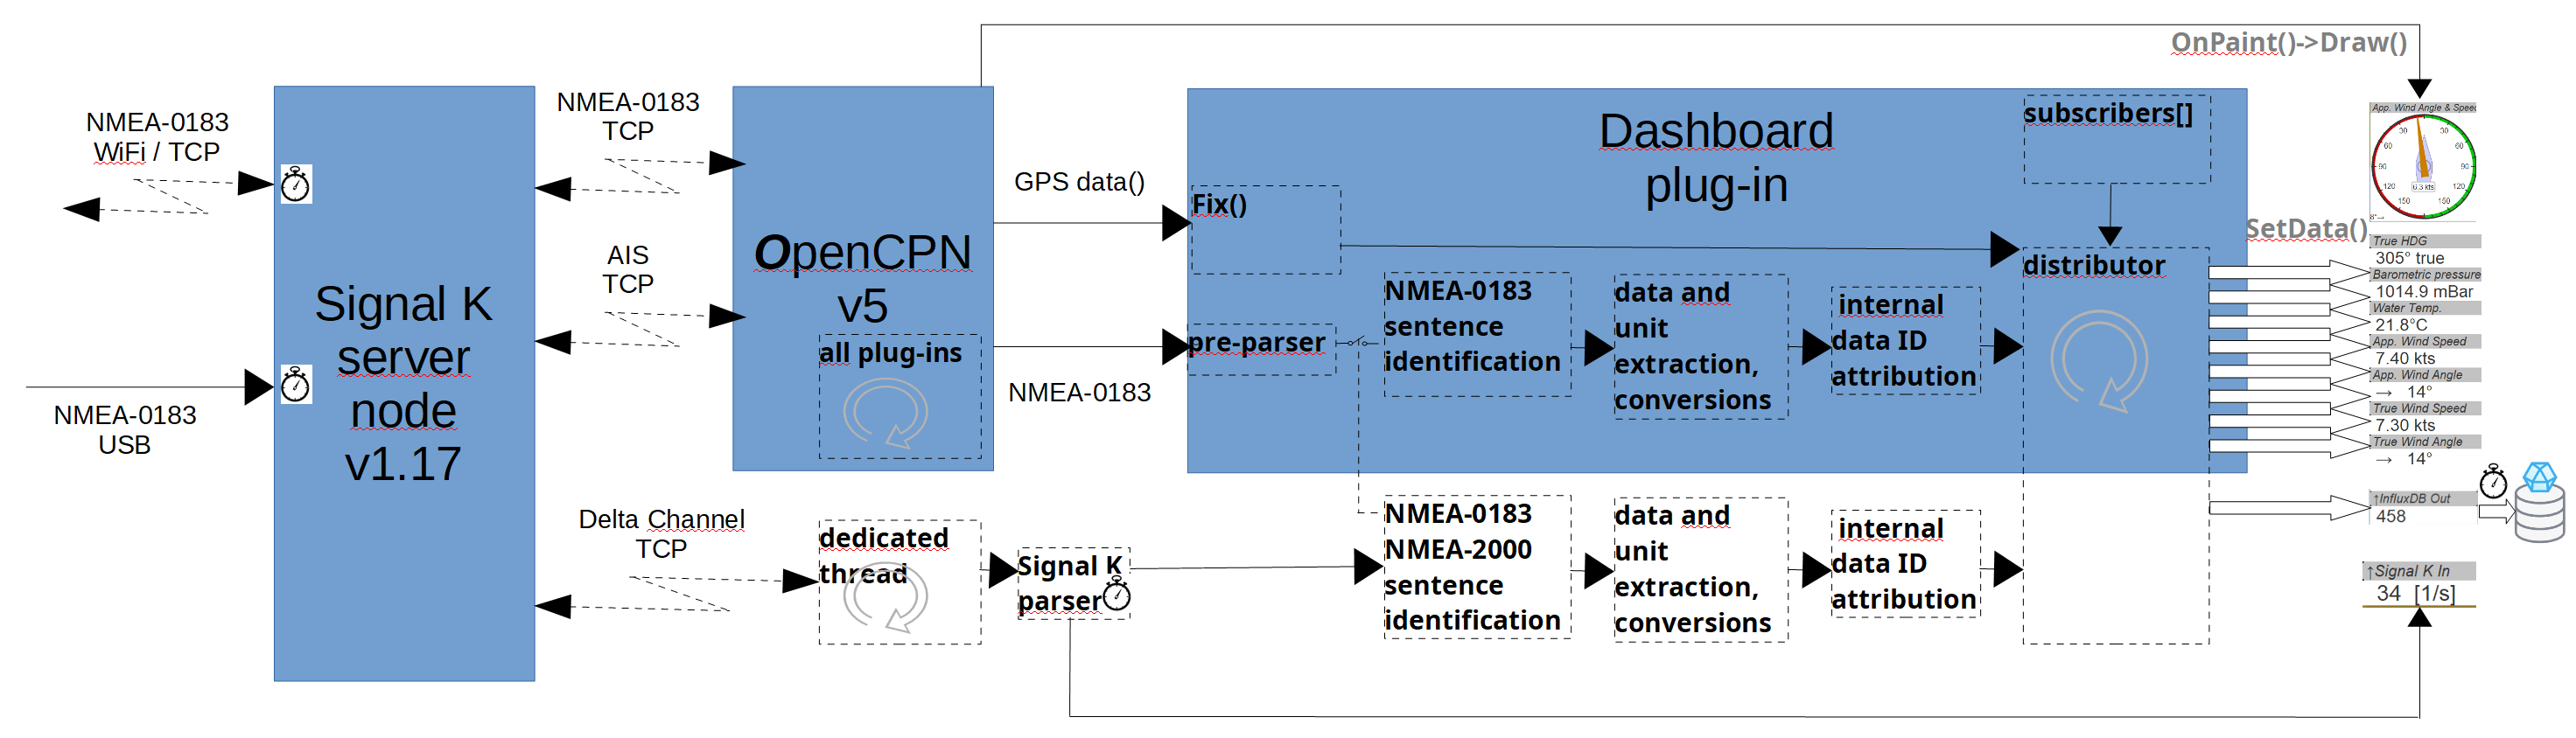
\includegraphics{signalkin-instrudiagram-3.png}
\href{img/signalkin-instrudiagram-3.png}{(zoom)}

    We could have written our own socket server if the requirement would
have been only to have timestamps at the arrival of data. However, when
we add the requirement to support not only NMEA-0183 but also NMEA-2000,
the choice of a Signal K server node is clear. The ligtweight and robust
server based on \emph{Node.js} is fast and stable. In addition it
provides additional services which we skip in this study. We use it to
feed the OpenCPN application which remains the distributor of NMEA-0183
sentences to plug-ins.

    In addition it feeds a \emph{joinable} wxWidgets thread which is
available continuously to serve the socket. This is advantageous
compared to the OpenCPN distribution model, since we are detached from
it and therefore independent from other plug-ins which may have been
subscribed to NMEA-0183 data.

    The thread contains a built-in parser of the Signal K data: the socket
is listening the so-called
\href{https://signalk.org/specification/1.3.0/doc/data_model.html\#delta-format}{delta
format} channel of Signal K which transmits a lightweight (relatively
speaking) data, or changes in it. The data is converted to simple
expression of C++ data types or wxWidgets string objects so that its
handling after this step will be extremely fast.

    After the parsing, we pass to a step by step structure, similar to the
one that already exists in Dashboard - the only difference is that now
the notion of NMEA-0183 specific sentences has disappeared - the data
can be either of NMEA-0183 or NMEA-2000 origin, the chain decides based
on Signal K schema to which instruments the data should be distributed.

    \begin{quote}
\textbf{Note}: this allows to add relatively easily (coding still
needed) new instruments which are dedicated to the engine control. As a
proof of concept, three such a engine control instruments have been
added into Dashboard-Tactics for engine speed, cooling water temperature
and oil pressure.
\end{quote}

    There is a software switch with a timeout: if the data is not available
from the Signal K input socket thread, or if there is no equivalent data
than in the Signal K delta data for a NMEA-0183 sentence, the software
switch closes and let the NMEA-0183 sentence to be passed to the
instruments.

    One of these instruments receiving the data can be - if user so wish -
Influx DB output stream. Now the data has the timestamp of when it
arrives into the system, not the time of when it was received by the
instrument.

    The timestamp is distributed to all instruments which are subscribed to
a given data and they can use it for new purposes which did not exist
before. For example, all instrument base classes contain now a default
behavior what shall happen if no new data is received within a timeout
period. This goes beyond Dasboard plug-in's own timeout with data
invalidation which is only applicable for some data classes, like GPS
data.

    Let's observe the new thread both in the Raspberry (Linux) and Windows
10 systems:

    \begin{figure}
\centering
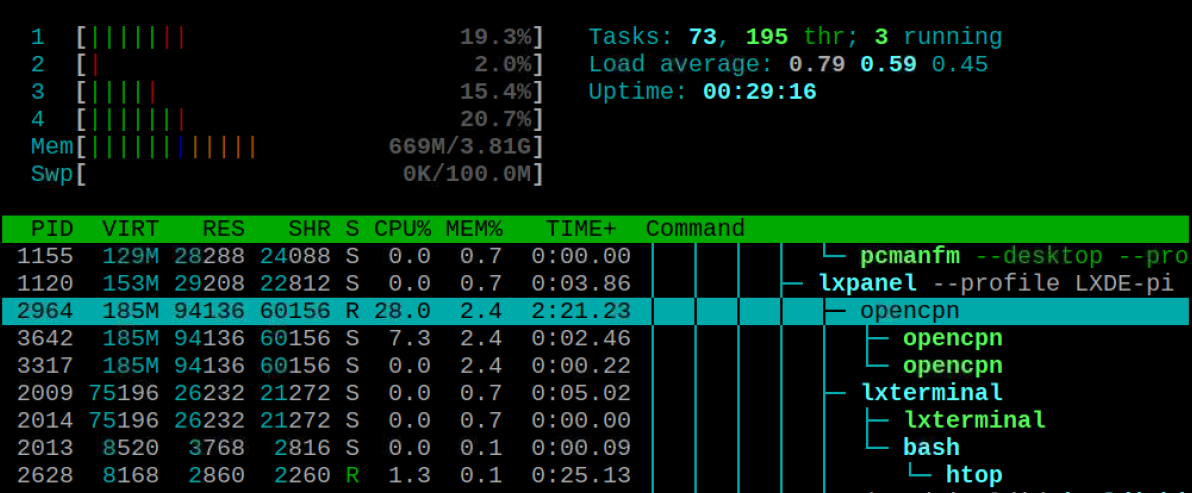
\includegraphics{2019-10-12_182800_rasbian_ov50_Influxdbout_signalkin_TCP_input_2_posix_threads.png}
\caption{2019-10-12\_182800\_rasbian\_ov50\_Influxdbout\_signalkin\_TCP\_input\_2\_posix\_threads.png}
\end{figure}

    \begin{figure}
\centering
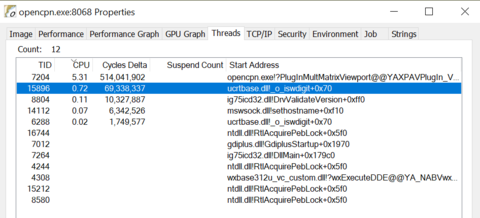
\includegraphics{2019-10-12_211324_w10_ov50_influxdbout_signalkin_TCP_threads.png}
\caption{2019-10-12\_211324\_w10\_ov50\_influxdbout\_signalkin\_TCP\_threads.png}
\end{figure}

    We can observe above the increased CPU load. This socket thread is doing
something! Let's observe does it translate as increased number of I/O
operations:

    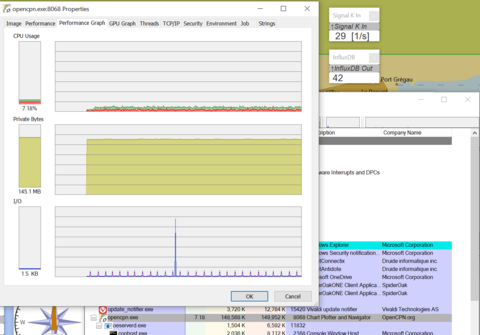
\includegraphics{2019-10-12_211323_w10_ov50_influxdbout_signalkin_TCP_perfgraph.png}
\href{img/2019-10-12_211323_w10_ov50_influxdbout_signalkin_TCP_perfgraph.png}{(zoom)}

    Yes! Please zoom in and you can see that there is clear increase in the
overall I/O operations, about 500 kB delta/s caused by the new channel
of data, Signal K delta data.

    \begin{quote}
\textbf{Note}: the payload of the Signal K delta data is by no means
containing strictly and only the data which the instruments need: it is
the delta of all data Signal K has got and therefore contains data which
is certainly not used by any instrument. The Signal K data format in
JSON is compact but still human readable and as such it is much longer
than the cryptic but compact NMEA-0183 data. However, this has not much
impact of today's fast communication channels since we are talking about
TCP/IP sockets here and not some RS-232-C 4800 baud line which, for all
practical purposes NMEA-0183 is.
\end{quote}

    \hypertarget{detailed-performance-analysis-of-the-implementation}{%
\subsubsection{Detailed performance analysis of the
implementation}\label{detailed-performance-analysis-of-the-implementation}}

    A set of example data was collected in real-life condition (in a boat
with the above configuration) for three use cases, both in a USB
connected Raspberry system and in a USB connected Window 10 system. No
WiFi was used but all TCP/IP connections were internal TCP/IP which, in
Linux means that the message is not passing through the device driver
stack.

    The detailed reports can be read using the below links.

    \emph{Raspberry Pi results}
(\href{analysis/Three-way_timestamps/Three-way_timestamps_Rpi.ipynb}{ipynb}
\textbar{}
\href{analysis/Three-way_timestamps/Three-way_timestamps_Rpi.html}{html}
\textbar{}
\href{analysis/Three-way_timestamps/Three-way_timestamps_Rpi.pdf}{pdf})

    \emph{Windows 10 results}
(\href{analysis/Three-way_timestamps/Three-way_timestamps_win10.ipynb}{ipynb}
\textbar{}
\href{analysis/Three-way_timestamps/Three-way_timestamps_win10.html}{html}
\textbar{}
\href{analysis/Three-way_timestamps/Three-way_timestamps_win10.pdf}{pdf})

    \hypertarget{conclusion}{%
\subsection{Conclusion}\label{conclusion}}

    The implementation meets the requirements. The obtained improvements in
the stability and in the reduction of the jitter are significant.

    There is performance margin which allows the boat owner to take
advantage of the modern socket based communication by increasing the
sampling rate of his or her sensors and instruments (by replacing them).

    The implementation enables the shortest possible data path to
instruments and, also importantly to Tactics ``regatta computer'' or
other algorithms, it enables greater data throughput with accurate
timestamps.


    % Add a bibliography block to the postdoc
    
    
    
\end{document}
